\documentclass[a4paper,14pt]{extarticle}
\usepackage{../../tex-shared/preamble}

\renewcommand{\mylabnumber}{1}
\renewcommand{\mylabtitle}{Манипулирование базой данных.
                           Реляционная алгебра и SQL}
\renewcommand{\mysubject}{Управление данными}
\renewcommand{\mylecturer}{Заикина Е.Н.}

\begin{document}
\begin{titlepage}
    
    \thispagestyle{empty}
    
    \begin{center}
        
        Министерство науки и Высшего образования Российской Федерации \\
        Севастопольский государственный университет \\
        Кафедра ИС
        
        \vfill

        Отчет \\
        по лабораторной работе №\mylabnumber \\
        \enquote{\mylabtitle} \\
        по дисциплине \\
        \enquote{\MakeTextUppercase{\mysubject}}

    \end{center}

    \vspace{1cm}

    \noindent\hspace{7.5cm} Выполнил студент группы ИС/б-17-2-о \\
    \null\hspace{7.5cm} Горбенко К. Н. \\
    \null\hspace{7.5cm} Проверил \\
    \null\hspace{7.5cm} \mylecturer

    \vfill

    \begin{center}
        Севастополь \\
        \the\year{}
    \end{center}

\end{titlepage}

\section{Цель работы}
Изучить основы реляционной алгебры как базового средства манипулирования.
Научиться представлять запросы как на реляционной алгебре, так и на SQL.

\section{Задание на работу}
Задана следующая схема БД:
\begin{figure}[H]
    \centering
    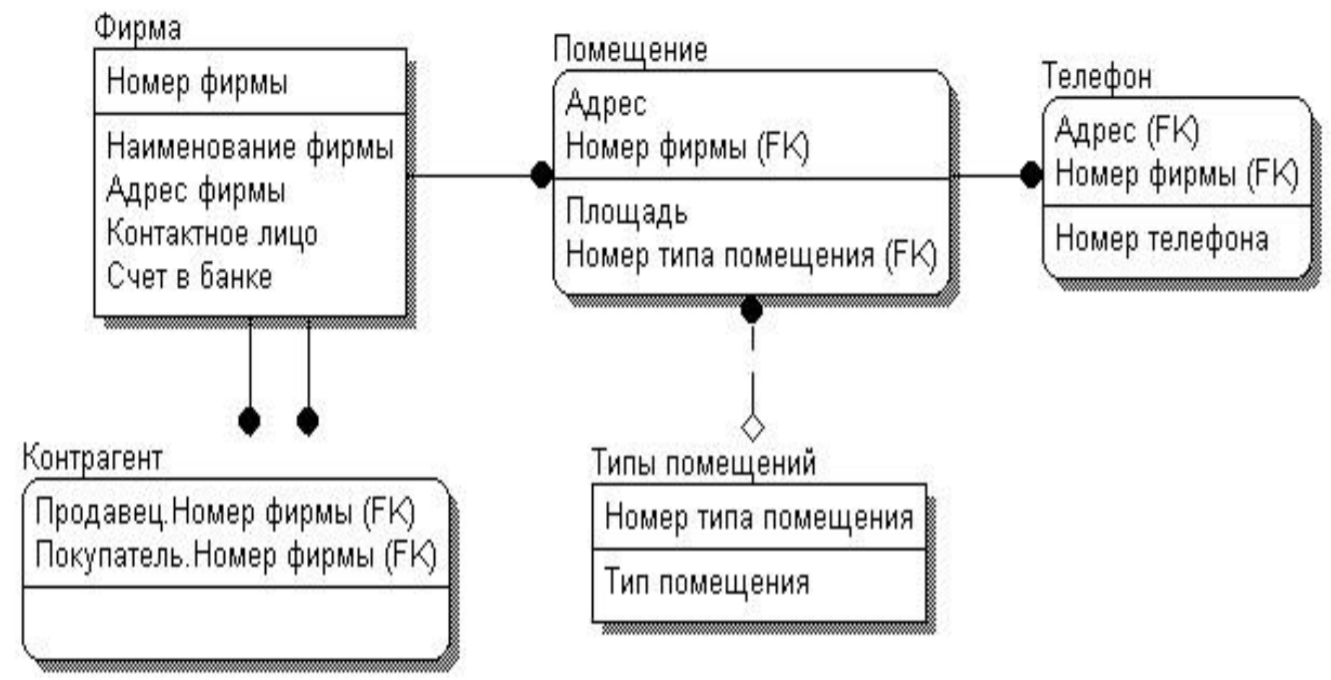
\includegraphics[width=.8\linewidth]{schema}
    \caption{Схема базы данных}
    \label{ref:schema}
\end{figure}

Для данной схемы выполнить следующие пункты:
\begin{enumerate}
    \item Создать базу данных и все ее таблицы. Заполнить базу данными.
    \item Продемонстрировать выполнение простых вычислений в запросе.
    \item Продемонстрировать работу предложений GROUP BY и HAVING.
    \item Применить к БД операции селекции и соединения в одном запросе.
    \item Создать запрос, использующий операции проекции и деления (в одном запросе).
    \item Создать запрос, использующий операции проекции, объединения и
          конъюнкции (в одном запросе).
    \item Создать запрос, использующий операции соединения и деления (в одном
          запросе).
    \item Создать запрос, использующий операции вычитания и дизъюнкции (в одном
          запросе).
    \item Сформулировать и записать запрос на SQL, не реализующийся на РА.
\end{enumerate}

\section{Ход работы}
Создадим базу данных по данной схеме. Атрибут \enquote{Номер телефона}
из таблицы \enquote{Телефон} переместим в таблицу \enquote{Помещение}
т.к. вынесение этого атрибута в отдельную таблицу смысла не имеет.

Для полученной базы выполним запросы:
\subsection{Выполнение простых вычислений, предложений \code{GROUP BY}, \code{HAVING}}
Для демонстрации простых вычислений выполним следующий запрос:
\begin{lstlisting}
SELECT 5 + 10 * 5;
\end{lstlisting}

Результат:
\begin{table}[H]
    \caption{Результат выполнения запроса}
    \noindent\begin{tabular}{|r|l|}
        \hline
        № & (No column name) \\ \hline
        1 & cell \\
        \hline
    \end{tabular}
\end{table}

Для демонстрации простых вычислений как параметров агрегатных функций,
предложений \code{GROUP BY} и \code{HAVIND}:
\begin{lstlisting}
USE TC;

SELECT [RoomTypeId], MIN([Area] * [RoomTypeId]) AS [MinArea*RoomTypeId]
FROM Quarters
GROUP BY [RoomTypeId]
HAVING MIN([Area] * [RoomTypeId]) < 1000;
\end{lstlisting}

Результат:
\begin{table}[H]
    \caption{Результат выполнения запроса}
    \noindent\begin{tabular}{|r|l|l|}
        \hline
        № & RoomTypeId & MinArea*RoomTypeId \\ \hline
        1 & 1 & 162 \\ \hline
        2 & 2 & 800 \\ \hline
        3 & 4 & 200 \\ \hline
    \end{tabular}
\end{table}

\subsection{Запрос с соединением и селекцией}
Для демонстрации соединения и селекции в одном запросе выполним следующий
запрос: выбрать информацию о компаниях, которые имеют помещения с площадью
менее 500.

Запрос на языке РА:

$R_{1} = Company \bowtie_{Id = CompanyId} Quarters;$

$R = R_{1} \sigma _{Area < 500};$

\begin{lstlisting}[language=SQL]
USE TC;

SELECT [c].[Id] AS [CompanyId], 
	   [c].[Name], 
	   [q].[Address],
	   [q].[Area],
	   [q].[RoomTypeId]
FROM [Company] AS [c] INNER JOIN [Quarters] AS [q] ON [c].[Id] = [q].[CompanyId]
WHERE [Area] < 500;
\end{lstlisting}

Результат:
\begin{table}[H]
    \caption{Результат выполнения запроса}
    \noindent\begin{tabular}{|r|l|l|l|l|l|}
        \hline
        № & CompanyId & Name	  & Address	                         & Area & RoomTypeId \\ \hline
        1 & 6         & Microsoft & Sevastopol, Bolshaya Morskaya, 4 & 400  & 2          \\ \hline
        2 & 12        & Foxconn   & Sevastopol, Gogolya, 24          & 162  & 1          \\ \hline
        3 & 5         & SpaceX    & Sevastopol, Hrustaleva, 3        & 252  & 1          \\ \hline
        4 & 1         & SevStar   & Sevastopol, Kolobova, 50         & 50   & 4          \\ \hline
        5 & 8         & Walmart   & Sevastopol, Lenina, 15           & 250  & 5          \\ \hline
        6 & 9         & Amazon	  & Sevastopol, Lenina, 25           & 140  & 4          \\ \hline
        7 & 4         & JetBrains & Sevastopol, Lenina, 3            & 123  & 4          \\ \hline
        8 & 2         & Sevsu	  & Sevastopol, Pozharova, 12        & 452  & 6          \\ \hline
    \end{tabular}
\end{table}
\end{document}